\subsection{SQLNet} \label{sec:sqlnet}

The model was designed to demonstrate that reinforcement learning should be limited to Text-to-SQL tasks.
Until SQLNet\cite{xu_sqlnet_2017}, all previous models used reinforcement learning to improve the decoder results when it generated appropriate serializations.


In cases where the order is irrelevant, SQLNet avoids the seq2seq structure.
For making predictions, the model uses a sketch-based approach consisting of a dependency graph that allows previous predictions to be taken into account.
The model also incorporates column attention (weights assigned to significant words and phrases in sentences) to improve the results. According to the flowchart below, SQLNet employs three phases to generate SQL queries for WikiSQL tasks.

% add image sqlnet.png
% \begin{figure}[htb]
%     \centering
%     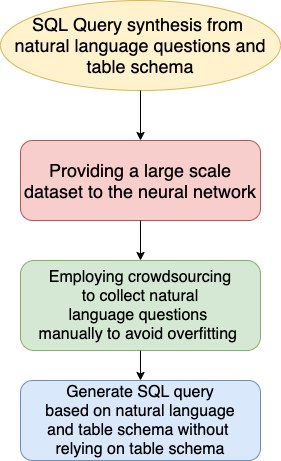
\includegraphics[width=0.3\textwidth]{pics/sqlnet/sqlnet.png}
%     \caption{SQLNet\cite{xu_sqlnet_2017}}
%     \label{fig:sqlnet}
% \end{figure}

\subsubsection*{Sketch-based query synthesis}

The token with the \$ sign represents an empty slot, and the token name represents the type of prediction. Tokens in bold represent SQL keywords such as SELECT, WHERE, etc.
\$AGG can be filled with either an empty token or one of the aggregation operators, such as SUM or MAX. Fill in the \$COLUMN and \$VALUE slots with the column name and substring of the question, respectively. The \$OP slot can be a value between \{=, \}. The notion \(...\)* uses a regular expression to indicate zero or more AND clauses.

\begin{figure}[htb]
    \centering
    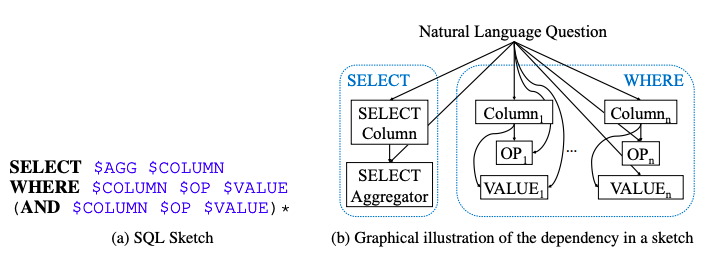
\includegraphics[width=0.8\textwidth]{pics/sqlnet/sketch-based.png}
    \caption{Sketch-based query synthesis\cite{xu_sqlnet_2017}}
    \label{fig:sketch-based}
\end{figure}

% bold text
\subsubsection*{Column attention for sequence-to-set prediction}

Instead of producing a sequence of column names, sequence-to-set prediction predicts the names of the columns of interest.
Based on column names, column attention is part of the generic attention mechanism for computing the feature attention map on a question.

\subsubsection*{Predicting WHERE and SELECT clause}

One of the most challenging tasks in Text-to-SQL is predicting the WHERE clause.
According to SQL sketch, SQLNet finds the columns that appear in the WHERE clause and predicts the OP slots and value for each column.

It is predicted that the OP slot will be filled with one of the three classes \{<,>,=\}, and the VALUE slot will be filled with the substring from the natural language question.
In SELECT clauses, columns are named, and aggregator functions are specified, such as count, sum, max, etc. There is only one difference between SELECT and WHERE: the column name. There is only one column selected in SELECT.

In the WikiSQL test set, SQLNet accuracy is 64.4\%, and in the SPIDER test set, it is around 12.4\%.

\begin{figure}[htb]
    \centering
    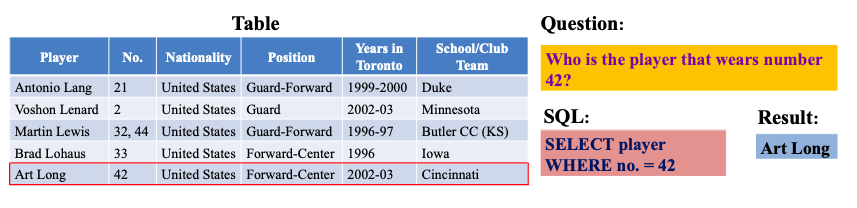
\includegraphics[width=0.8\textwidth]{pics/sqlnet/sqlnet-task.png}
    \caption{An example of a query executed by SQLNet on WikiSQL\cite{xu_sqlnet_2017}}
    \label{fig:sqlnet-task}
\end{figure}